En este capítulo se realiza una breve descripción del estado actual de la interacción hombre máquina, la interpretación del lenguaje natural y diferentes técnicas para aplicar estos principios a la creación de chatbots. Por otra parte, también se exponen distintas características sociales y de interacción a tener en cuenta en el diseño de un chatbot. Por último, se revisan varios casos de asistentes conversacionales orientados al campo de la salud y se exponen distintas herramientas disponibles para realizar una implementación.\\

\section{Interacción hombre-máquina y lenguaje natural}
%El lenguaje es la capacidad que tiene el ser humano para expresarse y comunicarse a través de diversos sistemas de signos orales, escritos o gestuales. De entre ellos el habla es posiblemente el más complejo pues actúa a diferentes niveles: semántico, lingüístico, articulatorio y sonoro \cite{designTechniques}. Como parte de. Entender correctamente el texto resultante es una tarea igualmente ardua pues el lenguaje va más allá del significado literal de las palabras y por tanto se requiere también una comprensión del contexto en el cual se desarrolla una conversación para interpretarlo correctamente.\\

El lenguaje es la capacidad que tiene el ser humano para expresarse y comunicarse a través de diversos sistemas de signos orales, escritos o gestuales. Con la aparición de nuevas tecnologías y la creciente capacidad de computación se han abierto nuevos campos de investigación de técnicas para el procesamiento de este lenguaje natural (\textit{NLP: Natural language processing}) con el propósito de utilizarlo como medio de interacción entre el hombre y máquina. En los últimos años estos esfuerzos se han materializado en el desarrollo de varios sistemas capaces de entender, hasta cierto punto, las intenciones expresadas por cualquier persona mediante su propia lengua para luego actuar en consecuencia. Si bien estos sistemas utilizan los últimos avances ofrecidos por la inteligencia artificial la realidad es que se encuentran aún en una etapa muy temprana de desarrollo. Por tanto, constituyen un punto de partida y sientan las bases del futuro de la interacción entre usuarios y dispositivos, estableciendo un escenario totalmente nuevo donde ya no será necesario utilizar ratón, teclado, pulsaciones o cualquier otro método tradicional de entrada. De hecho, las clásicas interfaces ya están dejando paso a un nuevo paradigma de interacción mucho más intuitivo dónde no es necesario hacer clicks ni teclear para realizar ciertas operaciones \cite{conversationSystems,shouldInteract}.\\

Por ejemplo, el asistente virtual \textit{Alexa} permite reproducir música con sólo decir \textit{Alexa, reproduce la lista relax de Spotify}. O \textit{Siri}, que puede encontrar la gasolinera más próxima a tu ubicación con un \textit{Oye Sire, indícame como ir a la gasolinera más cercana}. Aunque esto pueda parecer simple, ciertos procesos más complejos que antes podían resultar algo tediosos como reservar un vuelo, ahora ya son posible con un simple \textit{Google, resérvame un vuelo a París}, sin necesidad de navegar a través distintas webs ni rellenar formularios.\\

%\section{Reconocimiento de la intención}
%La intención representa el significado que hay detrás de un texto en lenguaje natural. En otras palabras, si se toma cualquier texto en lenguaje natural, la "intención" es la intención del escritor o hablante de ese texto, de ahí el término intención. El proceso de comprensión de la intención de una consulta del usuario se denomina reconocimiento de la intención y, en términos de programación, es un problema de clasificación. La clasificación se define como el problema de identificar a qué conjunto de categorías pertenece una nueva observación. En la clasificación de la intención, se tienen categorías de intención predefinidas y la tarea del bot es identificar la categoría de intención que mejor se ajusta a un nuevo texto en lenguaje natural que llega.

%\cite{buildingChatbots}

\section{Chatbots}
Un chatbot (\textit{chatter-bot}) o asistente virtual se puede definir como una interfaz (programa) diseñado para que los usuarios puedan interactuar con sus dispositivos haciendo uso de lenguaje natural, ya sea por voz o texto. El objetivo principal es siempre transmitir la sensación al usuario que se encuentra dialogando con una persona real y mantener esta ilusión el mayor tiempo posible. Para ello es crucial que los chatbots sean capaces de demostrar entendimiento, respondan con coherencia y resuelvan las tareas / problemas que los usuarios les planteen.\\

\subsection{Clasificación}
En los últimos años, con la popularización de los chatbots y la democratización de sus tecnologías se han creado multitud de \textit{bots} con propósitos muy distintos. Esto dificulta realizar una clasificación precisa dada la alta subjetividad respecto  al ámbito al cual puede pertenecer un chabot. Sin embargo, es posible realizar una clasificación general en función de los siguientes criterios: Objetivo, modo de interacción, técnica de diseño y ámbito \cite{designTechniques,chatbotTypes}.\\

\subsubsection{Objetivo (\textit{Goal})}
Según el objetivo para el cual han sido diseñados los chatbots pueden clasificarse en:

\begin{itemize}
  \item \textit{Task oriented}: Su objetivo es ayudar a los usuarios a realizar una tarea muy concreta \cite{designTechniques}. En consecuencia, están diseñados para desenvolverse en contextos bastante específicos como reservar un vuelo o anotar un evento en la agenda. En la mayoría de los casos estas acciones han sido establecidas previamente por lo que el flujo de la conversación y todos los posibles caminos están ya previstos \cite{chatbotTypes}.
  \item \textit {Non-task oriented / Conversacionales}: No tienen ningún propósito en particular y su función se limita a mantener una conversación con el usuario. Por ende, su propósito es asemejarse lo máximo a una conversación real respondiendo y siguiendo adecuadamente al interlocutor.
  \item \textit {Informativos}: Son \textit{bots} cuya única tarea es ofrecer al usuario la información que requiera. Normalmente esta información es extraída mediante algoritmos de \textit{string matching} de una base de datos u otra fuente de datos estática. Un ejemplo claro de aplicación son los asistentes que resuelven las dudas más frecuentes (\textit{FAQS}) \cite{chatbotTypes}.
\end{itemize}


\subsubsection{Modo de interacción}
Dependiendo de como el usuario interactúe con el asistente se puede clasificar el chatbot como basado en texto, basado en voz o en respuestas predefinidas. Los siguientes modos no son incompatibles y muchos \textit{bots} combinan ambos.


\begin{itemize}
	\item \textit{Voz}: Aquellos chatbots cuyo método de entrada es la voz. El asistente registra el conjunto de sonidos emitido por el usuario, lo traduce a texto e interpreta su significado. Este es el caso de los famosos asistentes del hogar como \textit{Google Home} o \textit{Alexa} dónde por la naturaleza de la aplicación el soporte de voz resulta ser lo más conveniente.
	\item \textit{Texto}: Los \textit{bots} basados en texto aceptan la escritura libre de cualquier mensaje y suelen encontrarse en dispositivos donde escribir resulta cómodo como ordenadores y móviles.
	\item \textit{Respuestas predefinidas}: Dentro de los chatbots basados en texto se encuentran aquellos con los que se interactúa mediante el uso de respuestas predefinidas, normalmente haciendo uso de botones de respuesta rápida. Estos asistentes tienen el flujo de conversación estrictamente definido y por tanto el usuario sólo puede recorrer un número limitado de caminos previamente definidos.
\end{itemize}



\subsubsection{Técnica de diseño}
\label{tecdis}
Para que un chatbot responda de forma adecuada es crucial reconocer que intenciones tiene el usuario cunado se expresa. Para ello, anteriormente se utilizaban algoritmos simples basados en reglas donde la interacción se limitaba a un simple patrón de pregunta-respuesta. Sin embargo, hoy en día con la aparición de nuevas técnicas es posible crear sistemas más complejos que nos permitan implementar patrones de conversación mucho más sofisticados, ofreciendo al usuario final una experiencia mucho más natural y humana. Actualmente existen múltiples técnicas de diseño para el desarrollo de chatbots:

\begin{itemize}
	\item \textit{Parsing}: Es un método que toma como valores de entrada el texto proporcionado por el usuario y extrae la información más significativa \cite{designTechniques}. Para ello, transforma el texto en un conjunto más sencillo de guardar y manipular. Actualmente, existen técnicas más avanzadas de \textit{parsing} que convierten el texto en una representación numérica entendible por los ordenadores.
	\item \textit{Pattern matching}: Es la técnica más empleada en el desarrollo de la mayoría de chatbots, sobretodo en los chatbots destinados a responder preguntas (\textit{QA chatbots}) \cite{designTechniques,conversationSystems}. Este método toma el \textit{input} generado por el usuario e intenta clasificarlo como uno de los patrones que ya tiene definidos. Una vez clasificado como \textit{pattern}, devuelve la respuesta asociada (\textit{template}). Estas relaciones \textit{pattern-response} se construyen a mano y constituyen uno de los principales inconveientes de estos sistemas \cite{designTechniques}. Aunque las técnicas de \textit{pattern matching} han estado presentes desde los primeros chatbots, han ido evolucionando hasta incluir cierta noción del contexto conversacional en sus algoritmos \cite{designTechniques}. 
	\item \textit{AIML}: AIML (\textit{Artificial Intelligence Mark-up Language}) es un lenguaje de marcas derivado de XML diseñado para representar el conocimiento que se le da a los chatbots \cite{conversationSystems}. AIML contiene los denominados \textit{AIML objects}, los cuales estan compuestos por \textit{topics} o \textit{categories}. Estos últimos son la unidad de información más importante de AIML. Están compuestos por dos elementos: \textit{pattern} y \textit{template}. El \textit{pattern} representa el \textit{input} del usuario y \textit{template} la respuesta asociada a esa entrada. El propósito de estos objetos es modelar el flujo conversacional.
	\item \textit{Chatscript}: Es una herramienta \textit{opensource} que combina un motor de comprensión del lenguaje natural y un sistema de control de diálogo. Esta diseñada para construir chatbots que puedan mantener conversaciones interactivas guardando el estado del usuario entre conversaciones \cite{designTechniques}. Para ello, utiliza un sistema de ficheros con reglas, las cuales se utilizan para definir el flujo del diálogo.
	\item \textit{Ontologías}: Las ontologías se utilizan en los chatbots para sustituir el conocimiento elaborado a mano, por el conocimiento ontológico \cite{designTechniques}. La mayor ventaja de esta técnica es la capacidad de los chatbots de establecer relaciones entre los conceptos de un dominio o área de conocimiento, pudiendo llegar a crear nuevos razonamientos \cite{designTechniques}.
	\item \textit{Markov Chain Model}: \textit{Markov Chain Model} es un modelo de probabilidad diseñado para predecir el siguiente estado en base al estado actual \cite{designTechniques}. Esto implica que, cada vez que el chatbot responde, construye una nueva frase en base al modelo probabilístico. Este sistema es una simplificación de un proceso más complejo de toma de decisiones, y por tanto, no funciona bien para emular conversaciones complejas. Sin embargo, es bastante popular para chatbots orientados al entretenimiento, donde basándose en el \textit{input} del usuario pueden imitar conversaciones simples \cite{designTechniques}. 
	\item \textit{Redes neuronales}: Hoy en día, con los últimos avances en \textit{machine learning}, y en especial, con las redes neuronales, ha sido posible desarrollar chatbots más inteligentes \cite{designTechniques}. La principal diferencia con los algoritmos basados en reglas es la capacidad de estos sistemas para aprender y mejorar. De hecho, en el campo del \textit{deep learning} se han desarollado sistemas neuronales capaces de aprender sin de datos sin etiquetar y sin supervisión. Esto ha provocado un creciente desarrollo de redes neuronales aplicadas al procesamiento del lenguaje natural, especialmente la red neuronal recurrente (RNN) y las redes de memoria a largo plazo (LSTM) \cite{designTechniques}.
\end{itemize}

\subsubsection{Ámbito}
En función del conocimiento que posea el chatbot y los campos que intente abarcar se pueden definir como de ámbito abierto o cerrado.

\begin{itemize}
	\item \textit{Ámbito  abierto}: Asistentes que no tienen una área de conocimiento en específico, tienen un carácter más general y suelen estar hechos para el entretenimiento.
	\item \textit{Ámbito cerrado}: Centrados en resolver dudas o realizar tareas dentro de un ámbito muy específico. Suelen  fallar al responder sobre temas más generales.
\end{itemize}


\begin{figure}[htbp]
\centering
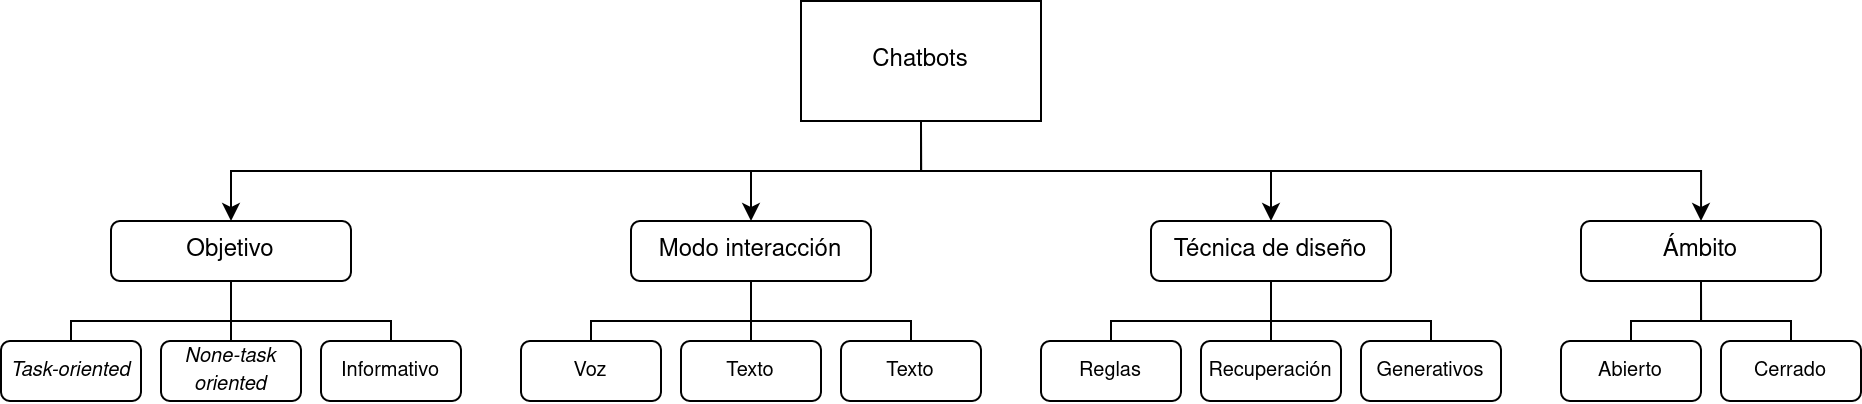
\includegraphics[scale=0.25]{../images/clasificacionChatbots.png} 
\caption{Clasificación de chatbots}
\label{fig:x clasificacion chatbots}
\end{figure}

 
 
%\subsection{Técnicas de diseño}
%\label{tecnicas diseño}
%Para que un chatbot responda de forma adecuada es crucial reconocer que intenciones tiene el usuario cunado se expresa. Para ello, anteriormente se utilizaban algoritmos simples de \textit{pattern matching} para construir sistemas basados en reglas donde la interacción se limitaba a un simple patrón de pregunta-respuesta. Sin embargo, hoy en día con la aparición de nuevas técnicas es posible crear sistemas más complejos que nos permitan implementar patrones de conversación mucho más sofisticados, ofreciendo al usuario final una experiencia mucho más natural y humana. \\

%la inteligencia artificial nos ha brindado una serie de herramientas muy útiles para para este objetivo: la comprensión del lenguaje natural, consciente del contexto, \textit{machine learning} y  aprendizaje supervisado. \\

%[TODO: Desarrollar técnicas de diseño]


\subsection{Interacción y características sociales}
\label{interaccion}
Como ya se ha mencionado, es de vital importancia que las conversaciones entre el \textit{bot} y el usuario sean lo más semejantes posibles a una entre humanos. Para ello no deben de transmitir una sensación robótica, si no que deben ser fluidas y lo más naturales posibles. Para ello, un chatbot debe de integrar una serie de rasgos que garanticen esta experiencia.\\

Estas características sociales han sido extraídas del artículo \textit{How should my chatbot interact? A survey on social characteristics in human-chatbot interaction design} \cite{shouldInteract} de Ana Paula Chaves y Marco Aurelio Gerosa. En él, se hace un repaso a la literatura actual sobre cómo debería actuar un chatbot, que rasgos de personalidad debería tener y diferentes comportamientos observados. A continuación se describen aquellos aspectos que se han considerado más relevantes.\\

\subsubsection{Proactividad}
La proactividad es la capacidad de un sistema de poder actuar autónomamente en nombre del usuario. Un comportamiento proactivo aporta iniciativa a una conversación, contribuyendo a sostener una conversación más natural. En un ámbito más práctico, los chatbots se pueden mostrar proactividad cuando sugieren nuevos temas, realizan preguntas y ofrecen información adicional.\\

\subsubsection{Conciencia}
La conciencia es la capacidad de un chatbot para demostrar atención y entendimiento en una conversación. Para ello es crucial que sepa interpretar el contexto, evaluando cada frase como parte de un conjunto. Cuando un chatbot no interpreta correctamente el significado o la intención de un mensaje, su credibilidad y humanidad se ve comprometida. 


\subsubsection{Comunicabilidad}
La comunicabilidad, en el contexto de los chatbots, es la capacidad de transmitir al usuario qué funcionalidades tiene. El uso de elementos visuales como respuestas rápidas e imágenes  pueden ayudar a mostrar al usuario qué tareas puede realizar el chatbot, y por tanto, reducir el número de errores de entendimiento. De hecho, un estudio realizado sobre chatbots relacionados con las noticias confirmó que el 63\% de las conversaciones con los chatbots se iniciaban haciendo click sobre un elemento mostrado en el mensaje inicial.\\

Por otra parte, el chatbot debe aclarar el objetivo del chatbot a través de un mensaje inicial y estar preparado para responder a preguntas como \textit{¿Qué puedes hacer?} o \textit{¿En qué me puedes ayudar?}.\\

\subsubsection{Controlar daños}
Todo asistente conversacional, por muy bien diseñado que esté, se enfrentará tarde o temprano a una situación no contemplada previamente. El control de daños (damage control ) son las diferentes técnicas que se pueden implementar para tratar de recuperarse en situaciones conflictivas o donde el chatbot falle. Por ejemplo, es común que un chatbot erre en una conversación debido a la falta de conocimiento lingüístico, o por enfrentarse a una pregunta que se encuentra fuera de su ámbito de conocimiento. Por tanto, un asistente debe ser capaz de reconocer estas situaciones, responder admitiendo su error e intentar reconducir la conversación.\\

Además, también debe detectar conductas abusivas y responder adecuadamente ante insultos y vejaciones, intentando evitar que el usuario continue con su conducta.\\ 

\subsubsection{Rigurosidad}
La sigurosisdad es la habilidad de un chatbot de ser preciso en la forma que utiliza el lenguaje. El lenguaje utilizado por un asistente debe ser consistente y no combinar varios estilos. Por ejemplo, muchos usuarios pueden ver extraño el uso combinado de emojis con un estilo muy formal.

\section{Chatbots en el campo de la salud}
Muchas de las tecnologías mencionadas anteriormente se han empezado a introducir en el campo de la medicina y de la salud en busca de soluciones que mejoren la vida de los pacientes. Aprovechando los últimos avances en interacción entre personas y máquinas  se están desarrollando propuestas de asistentes virtuales que ayuden en el día a día a pacientes, familiares o incluso personas mayores. La idea es siempre mejorar la atención y automatizar ciertos procesos médicos \cite{healthAgents} bastante comunes y rutinarios como puedan ser responder a ciertas consultas, realizar el seguimiento de una medicación o incluso detectar indicios de enfermedad. \\

Dependiendo de la intención y problema que pretendan solucionar en el campo se la salud se diferencian 4 grandes categorías: educación, \textit{coaching}, prevención y diagnóstico.\\

\subsubsection{Educación}
Los chatbots educativos son aquellos orientados a ayudar a los usuarios a entender conceptos médicos y resolver todas aquellas dudas que puedan tener. Esta tarea la pueden realizar proporcionando información relevante sobre cierta enfermedad, resolviendo dudas técnicas sobre un análisis o ayudando a pacientes y familiares a comprender diagnósticos y tratamientos. \\

Por ejemplo, un asistente virtual en este contexto podría resultar útil para  concienciar y advertir a la población sobre los riesgos de una determinada enfermedad. Este es el caso de IRA \cite{ira}, un chatbot creado en India que, al igual que VIHrtual-App tiene por objetivo ayudar con en el grave problema padece el país con el VIH ofreciendo información y motivando a la gente a ser conscientes y responsables (ver Figura \ref{fig:x captura ira}).\\

Dado  IRA comparte objetivos con VIHrtual-App, merece especial consideración hacer una breve descripción de sus principales características. Primeramente, y diferencia de VIHrtual-App, IRA no está diseñada para interactuar utilizando el idioma propio del país, si no que ha sido programado en inglés. Por tanto, su público o alcance es mucho mayor, pues cualquier usuario del mundo puede acceder e informarse. Por contra, presenta poca tolerancia a los errores gramaticales y no detecta muchas expresiones informales. También se ha observado que no es capaz de reconocer distintas variantes de una misma pregunta. Por ejemplo, en las pruebas realizadas, IRA identificó correctamente la expresión \textit{Risk of anal sex}, pero falló en reconocer otras expresiones como \textit{Is anal sex dangerous?} o \textit{Why is anal sex dangerous?}.\\

En este sentido, en el diseño propuesto para VIHrtual-App se incluye como requisito que el asistente robusto, sea capaz de detectar diferentes variaciones de una misma pregunta y entienda tanto un registro formal como informal.\\ 

\begin{figure}[htbp]
\centering
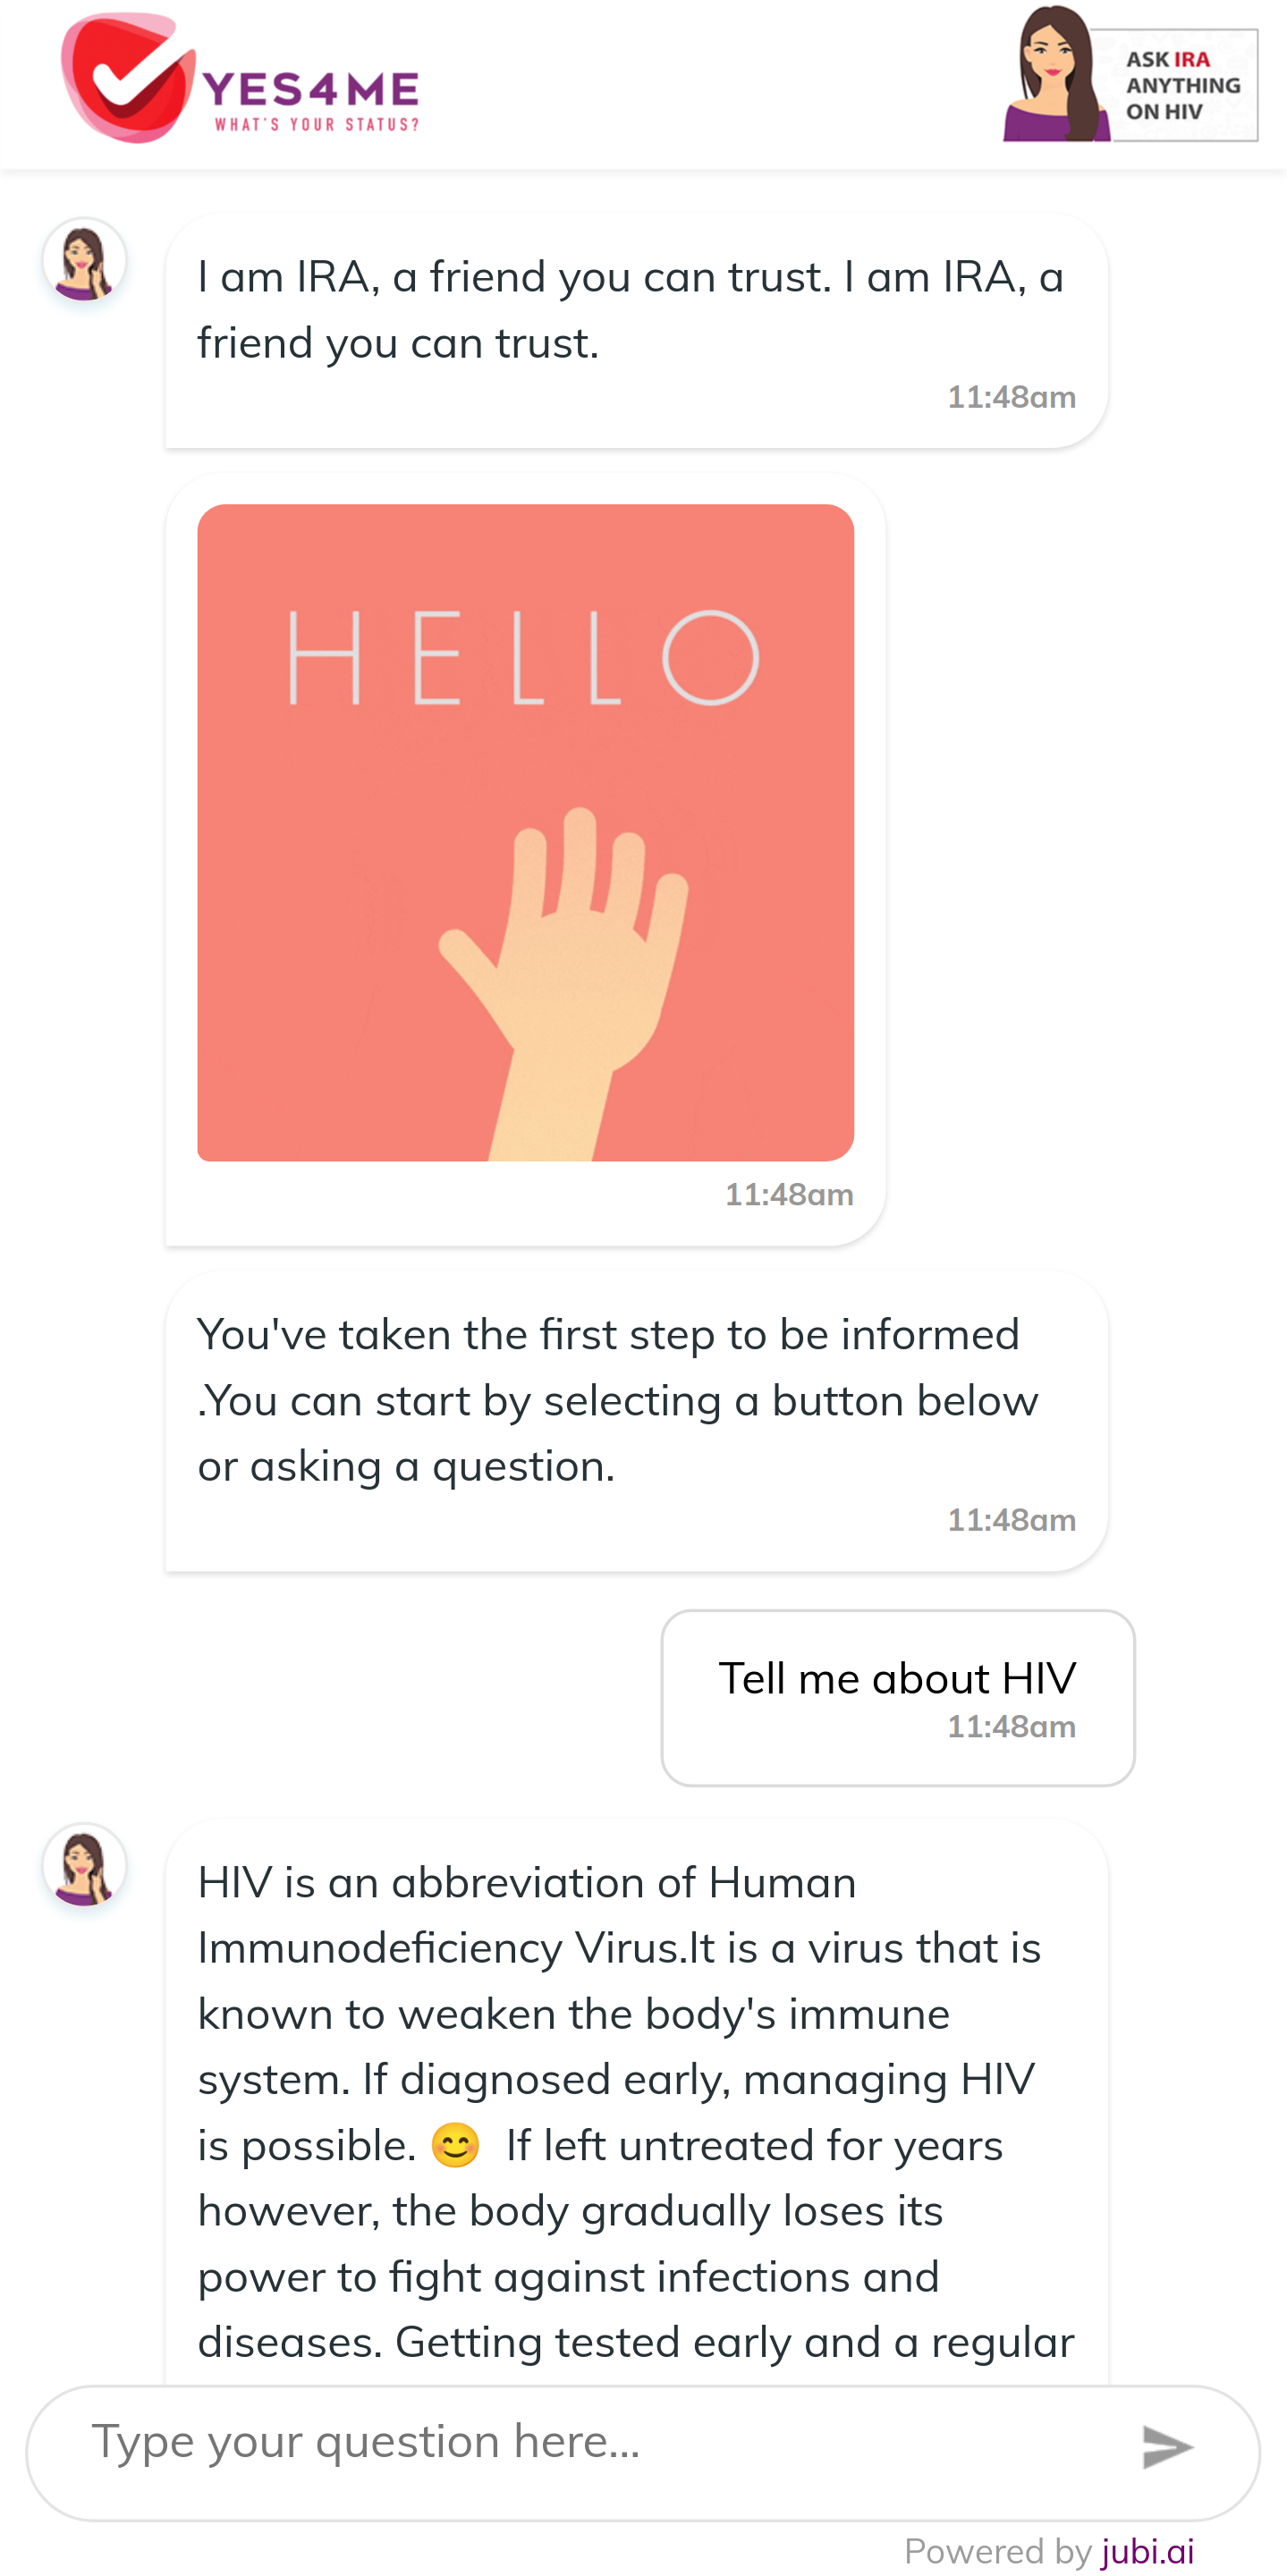
\includegraphics[scale=0.1]{../images/ira.png} 
\caption{Captura de pantalla de IRA}
\label{fig:x captura ira}
\end{figure}

\subsubsection{Coaching}
La segunda categoría hace referencia al término \textit{coach} (entrenador personal). Son chatbots similares a los anteriores pues están orientados también a formar al usuario pero, si en el anterior grupo la posición del asistente era bastante pasiva, aquí es todo lo contrario. Este tipo de asistentes toman una actitud de liderazgo para influir y mejorar directamente en la salud del usuario.\\

De esta manera, un chatbot podría enviar notificaciones al móvil de un paciente para recordarle cuándo debe tomar la medicación y así trabajar para introducir nuevos hábitos y comportamientos. También podría aconsejar mejores hábitos de vida y proponer objetivos diarios al usuario, trabajando codo con codo para mejorar su salud.\\

Un buen ejemplo de esta aplicación es Florence \cite{florence} (ver Figura \ref{fig:x captura florence}), un asistente que pretende ser un enfermero personal que recuerda a los usuarios cuándo deben tomarse la medicación y lleva un seguimiento del peso, presión arterial y periodo.\\

\begin{figure}[htbp]
\centering
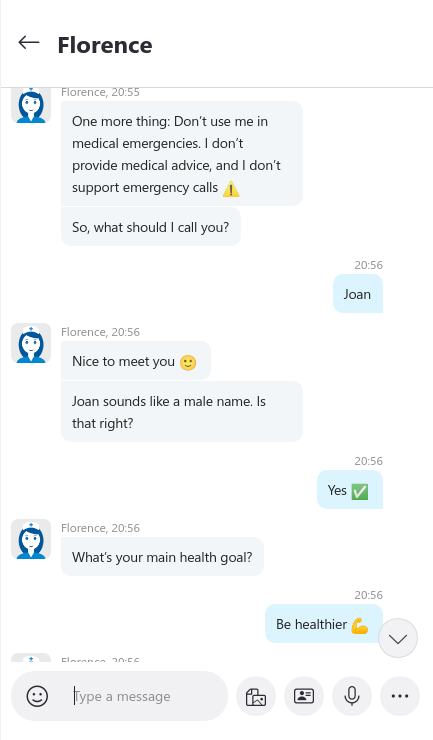
\includegraphics[scale=0.5]{../images/florence.png} 
\caption{Captura de pantalla de Florence}
\label{fig:x captura florence}
\end{figure}

\subsubsection{Prevención}
En la categoría de prevención se engloban todos aquellos chatbots orientados a mantener una relación continua entre médico y paciente. A través de conversaciones rutinarias un asistente virtual puede detectar patrones habituales ya conocidos y anticiparse a cualquier problema que pueda derivar en una posible enfermedad. Por ejemplo, mediante técnicas más avanzadas es posible detectar principios de demencia \cite{detectDementia} o actitudes depresivas para la prevención de suicidios.\\


\subsubsection{Diagnóstico}
Por último, el cuarto grupo son aquellos chatbots que en base a unas indicaciones sintomatológicas es capaz de sugerir un diagnóstico. Esta clase de \textit{bots} suelen utilizarse un ambiente clínico como una herramienta más para los médicos y que, por ejemplo, haciendo uso de grandes bases de datos y estadísticas sugieran al médico posibles diagnósticos.\\

Por otra parte también existen aplicaciones en este sentido donde se usa directamente por usuarios fuera del ámbito médico, y por tanto, suelen ser diagnósticos más sencillos. En esta dirección trabaja \textit{Wakamola} \cite{wakamola} (ver Figura \ref{fig:x captura wakamola}), un chatbot que, a través de una serie de preguntas recoge información sobre la dieta, actividad física, edad, peso etc. En función de las respuestas del usuario se realiza un cálculo y se muestra una puntuación (\textit{Wakaestado}) entre 0 y 100.

\begin{figure}[htbp]
\centering
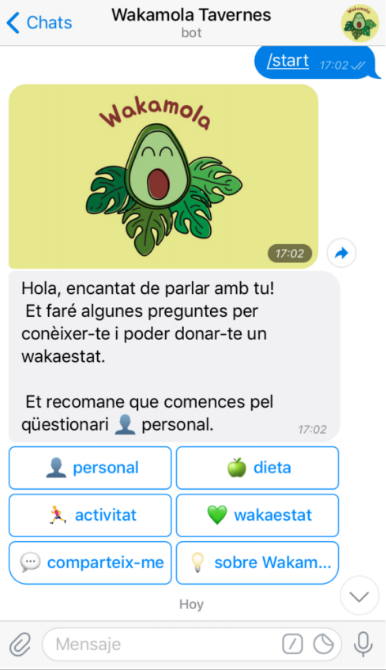
\includegraphics[scale=0.5]{../images/wakamola.png} 
\caption{Captura de pantalla de Wakamola}
\label{fig:x captura wakamola}
\end{figure}

\section{Herramientas para construir chatbots} \label{herramientas construir chatbots}
A la hora de desarrollar un chatbot existen diferentes herramientas que facilitan el uso e implementación de varias de las técnicas descritas en la sección \ref{tecdis}. A continuación se realiza un análisis y comparativa de las alternativas más relevantes para construir chatbots.\\

\subsection{Rasa}
\textit{Rasa} \cite{rasa} es un \textit{framework} gratuito y \textit{opensource} que permite construir sistemas conversacionales inteligentes. Esta herramienta proporciona tres grandes funcionalidades para la construcción de un chatbot: comprensión del lenguaje natural (\textit{NLU}), control del flujo los diálogos mediante algoritmos de \textit{machine learning} e integración con distintos canales (\textit{API REST}, aplicaciones de mensajería instantánea etc).\\

\textit{Rasa} hace una fuerte apuesta por el desarrollo basado en conversaciones reales (\textit{CDD: Conversation driven development}) y para ello ofrece un producto gratuito llamado \textit{Rasa X}. Aunque no es \textit{opensource} sí es gratuito y de libre uso facilitando la recogida y posterior etiquetado de las conversaciones.\\

\subsection{Amazon Lex}
Amazon Lex \cite{amazonlex} es un servicio para crear agentes conversacionales que interactúen mediante voz o texto. Esta tecnología es la misma que se encuentra detrás de \textit{Alexa}, por tanto este servicio pone a disposición de los desarrolladores el propio motor del popular asistente de Amazon.\\

Las principales características que ofrece son comprensión del lenguaje natural (NLU), reconocimiento automático de voz (ASR) e integración con distintos canales (aplicaciones de mensajería y web). El uso de la voz y la potencia de motor permite construir experiencias muy atractivas pero por contra, el servicio hace uso de los sistemas en la nube y cobra por cada solicitud de texto o voz que se realice (3.25\euro{} por cada 1000 peticiones de voz y 0.60\euro{} por cada 1000 de texto). \\


\subsection{Microsoft Bot Framework}
\textit{Bot Framework} es el producto ofrecido por \textit{Microsoft} para construir \textit{bots} conversacionales. Este servicio ofrece un conjunto de herramientas que interactúan su propia plataforma de computación en la nube \textit{Azure}. Por tanto, se trata de un servicio de pago que requiere de conexión para funcionar.\\

Sin embargo, cuenta con un plan gratuito y sin límite de mensajes, siendo la única limitación los canales por los cuales se puede acceder al chatbot. Los canales disponibles gratuitamente son \textit{Skype}, \textit{Slack}, \textit{Facebook}, \textit{Cortana} y \textit{MS Teams}. Si se desea conectarse al chatbot a través de otros canales, como por ejemplo una web, es necesario recurrir al pago del servicio (0.42\euro{} por cada 1000 mensajes).\\

\subsection{Botkit}
\textit{Botkit} \cite{botkit} es una herramienta \textit{opensource} para crear chatbots que puedan integrarse en aplicaciones web o en las principales plataformas de mensajería instantánea. Actualmente forma parte del conjunto de herramientas de \textit{Microsoft Bot Framework} por lo que ofrece soporte para hacer uso de \textit{LUIS.ai} \cite{luis}.\\

Por otra parte, \textit{Botkit} también ofrece una herramienta adicional denominada \textit{Botkit CMS}. Con ella, es posible diseñar, construir y gestionar diálogos de manera gráfica, permitiéndonos así crear interacciones más complejas donde el \textit{bot} pueda realizar preguntas o realizar distintas acciones. Junto con \textit{Rasa}, ambas son las dos grandes alternativas de código abierto para el desarrollo de chatbots. En comparación, \textit{Botkit} tiene un desarrollo bastante menos activo, siendo su última versión de hace aproximadamente un año. En cambio, \textit{Rasa} lanza versiones menores cada pocos meses y posee una comunidad más activa.\\


\subsection{Comparativa}
En la tabla \ref{compFrameworks} se puede observar una comparativa con las principales características de los \textit{frameworks} descritos anteriormente. Tras valorar las distintas alternativas para construir chatbots se escoge a \textit{Rasa} como plataforma sobre la cual se realizará el desarrollo. Las razones detrás de esta elección son las siguientes:\\ 

\begin{itemize}
	\item \textit{Rasa} cuenta con todas las herramientas necesarias para la correcta interpretación de las intenciones del usuario mediante técnicas de \textit{NLU} y noción del contexto.
	\item Es \textit{opensource}, gratuito y a diferencia de otros competidores, no se basa en ningún servicio en la nube propietario. Esto permite realizar el despliegue completo de la plataforma en cualquier máquina. 
	\item  En consecuencia, se obtiene independencia de otros servicios y control total sobre los datos recopilados de conversaciones, pues estas no estarán en manos de terceros.
	\item La plataforma ofrece una herramienta adicional para el aprendizaje supervisado llamada \textit{Rasa X}. Esta permite realizar fácilmente la revisión y etiquetado de las conversaciones por lo que resulta idónea para el desarrollo.
\end{itemize}	

\begin{table}[htbp]
\centering
\begin{tabular}{|l|l|l|l|l|} 
\hline
                   & Microsoft & Botkit   & Amazon Lex & Rasa      \\ 
\hline
Basado en la nube  & Sí        & No       & Sí         & No        \\ 
\hline
NLU                & Sí        & Sí       & Sí         & Sí        \\ 
\hline
Soporte mensajería & Sí        & Sí       & Sí         & Sí        \\ 
\hline
Coste              & Pago      & Gratuito & Pago       & Gratuito  \\
\hline
\end{tabular}
\caption{Comparativa de \textit{frameworks}}
\label{compFrameworks}
\end{table}
